\RequirePackage[T1]{fontenc}
\documentclass[journal]{IEEEtran}
\usepackage[T1]{fontenc}
\usepackage{amsmath,amssymb,amsthm,booktabs,graphicx,array,url}
\usepackage[hidelinks]{hyperref}
\ifdefined\XeTeXversion\AtBeginDocument{\special{pdf:minorversion 7}}\fi
\graphicspath{{figures/generated/}}
\newtheorem{proposition}{Proposition}
\newcommand{\E}{\mathbb{E}}
\newcommand{\R}{\mathbb{R}}
\newcommand{\FOneA}{0.9547}
\newcommand{\FOneB}{0.4555}
\newcommand{\FOneC}{0.7687}
\newcommand{\FOneD}{0.6458}
\newcommand{\FOneE}{0.9082}
\newcommand{\FOneF}{0.8535}
\newcommand{\FOneG}{0.8656}
\newcommand{\FOneH}{0.8646}

\title{Across the Proxy Boundary: Task-Dependent Traffic Correspondence and the Limits of Model Reuse}
\author{Research Draft---Author Information Withheld}
\markboth{RESEARCH DRAFT, SEPTEMBER 2026}{Across the Proxy Boundary}
\begin{document}
\raggedbottom
\maketitle
\begin{abstract}
Encrypted proxies alter traffic statistics while retaining some correspondence between observations on their two sides. Whether this correspondence enables a classifier trained at the proxy entrance to operate on exit-side traffic is less clear. We study this question through paired measurement and controlled model reuse, rather than assuming that recoverable traffic structure is automatically useful for classification. Our main cohort contains 240 visits to 30 contents across six domain--activity classes and two observed deployments, with five content-disjoint folds. A fixed source classifier achieves a macro-F1 of \FOneA{} on entrance observations but only \FOneB{} when directly applied to exit observations. Coordinate-wise statistical calibration recovers \FOneC{}. Adding a source-decision preservation objective, without increasing mapping capacity, raises macro-F1 to \FOneF{} even as statistical reconstruction error increases. Replacing visit-level targets with content--deployment centers further separates reconstruction fidelity from classification utility; its pooled performance is close to, but not established as equivalent to, instance-based controls. Finally, source-only fitting reveals asymmetric cross-deployment reuse and substantial degradation of the source classifier even on target-deployment entrance traffic. These results identify task objective, correspondence granularity, and deployment conditions as distinct constraints on exploiting paired traffic. They do not establish universal pairing benefits, deployment-invariant representations, or an index-free online attack.
\end{abstract}
\begin{IEEEkeywords}
Encrypted traffic analysis, proxy traffic, paired observations, model reuse, distribution shift, traffic measurement.
\end{IEEEkeywords}
\section{Introduction}
\IEEEPARstart{E}{ncrypted} communication hides payload content but leaves observable packet sizes, directions, and timing. Website fingerprinting demonstrates that these observations can support inference despite encryption~\cite{df,automated}. Flow-correlation research further shows that relationships between observations can be learned across a network path~\cite{deepcorr}. These findings motivate a different question for proxy traffic: can knowledge learned at one side of a proxy be reused when only the other side is available at inference time?

This question is not answered by high classification accuracy on either side alone. A model may distinguish deployments without identifying business activity. A feature may be accurately recoverable across sides while adding little to a particular classifier. Conversely, a mapping with imperfect reconstruction may preserve the relative class scores that matter to that classifier. Treating these properties as interchangeable risks attributing prediction improvements to a general invariant representation that has not been demonstrated.

Two challenges make the distinction operationally important. First, paired traffic shares workload, content, and visit-specific variation. Exact correspondence may expose any combination of these components, whereas a downstream label may distinguish only domain--activity classes. A correspondence objective can therefore favor faithfully preserving variation that is not essential to that classification problem. Second, the proxy entrance is not an environment-independent reference. Network feedback, implementations, and collection conditions can affect entrance traffic as well as exit traffic. Even perfect reconstruction of a target-deployment entrance representation does not guarantee that a source-deployment classifier will classify it correctly.

We address these challenges through a measurement-driven study with a fixed-capacity adaptation mechanism. We first characterize paired statistical changes and contrast feature recoverability with classification utility. We then retain a linear source classifier and compare direct application, coordinate-wise statistical calibration, and a calibration objective that also preserves centered source logits. Exact visit pairing, within-content cyclic mismatch, and content--deployment center targets isolate different uses of correspondence. Finally, we refit the complete pipeline on one deployment and evaluate held-out contents in the other deployment. This last experiment separates fit-time isolation from the historical fact that both deployments have already informed the research process.

The results show why a single ``pairing helps'' statement is insufficient. Under the same content partition, direct cross-side application reduces macro-F1 from \FOneA{} to \FOneB{}. Statistical calibration restores \FOneC{}, and decision-aware calibration reaches \FOneF{} with the same 298 mapping parameters. However, the decision-aware mismatched and center controls achieve \FOneG{} and \FOneH{}, respectively; the exact-target variant is not uniformly superior. Cross-deployment results are directional: calibration improves classification in the VLESS-to-SS direction, whereas the reverse direction chiefly improves probability loss. The target-entrance diagnostic also degrades in both directions.

Our contributions are threefold.
\begin{itemize}
\item We provide an auditable paired-traffic characterization that distinguishes repeatable statistical correspondence from finite-learner task utility, without using endpoint identity fields as predictor inputs.
\item We construct a fixed-source, fixed-capacity calibration study that separates recovery objective from correspondence granularity, retaining negative controls and deployment-specific exceptions.
\item We identify distinct cross-side and cross-deployment limits of model reuse through fit-time isolated evaluation and explicit observation permissions.
\end{itemize}
The contribution is the controlled empirical relationship among these properties. We do not claim a new information-theoretic identity, state-of-the-art classification, or an end-to-end operational attack.

\section{Background and Observation Model}
\subsection{Sides, Entities, and Labels}
We use \emph{pre} and \emph{post} for the paired entrance- and exit-side observation scopes defined by the collection index. Pre is traffic observed during a proxied session, not a separately captured direct connection without a proxy. A bidirectional TCP conversation is a connection; a unidirectional run consists of consecutive packets in one direction. The prediction unit is an indexed visit aggregating eligible, exclusive TCP pairs, not an individual connection or arbitrary sliding window.

The target label is domain $\times$ activity. The six primary classes are Bing search, MDN documentation, GitHub repository browsing, Wikipedia article browsing, YouTube search, and YouTube video playback. Each class contains five contents. Most domains contribute one activity, so the task is not platform-independent semantic activity recognition. The two YouTube classes provide a limited within-domain distinction, not an independent validation dataset.

\subsection{Training and Inference Permissions}
During development, paired visits provide pre and post statistics, content membership, and activity labels. These resources allow fitting a source classifier and a post-to-pre adapter. At inference, methods B--H use only the indexed post feature vector, except that A is a deliberately separate pre-side diagnostic. Evaluation subsequently reads labels and, for reconstruction diagnostics, held-out pre values. Test pre values never enter post prediction, normalization, target construction, or model selection in the frozen experiment.

The inference constraint concerns numerical prediction, not discovery of the traffic object. Eligible post objects are selected using offline collection indices. Thus the study uses an \emph{offline index-assisted post} observation model. It does not solve stream discovery, association of arbitrary background connections with a visit, or online segmentation without an index. Figure~\ref{fig:boundary} makes this distinction explicit.

\begin{figure*}[t]
\centering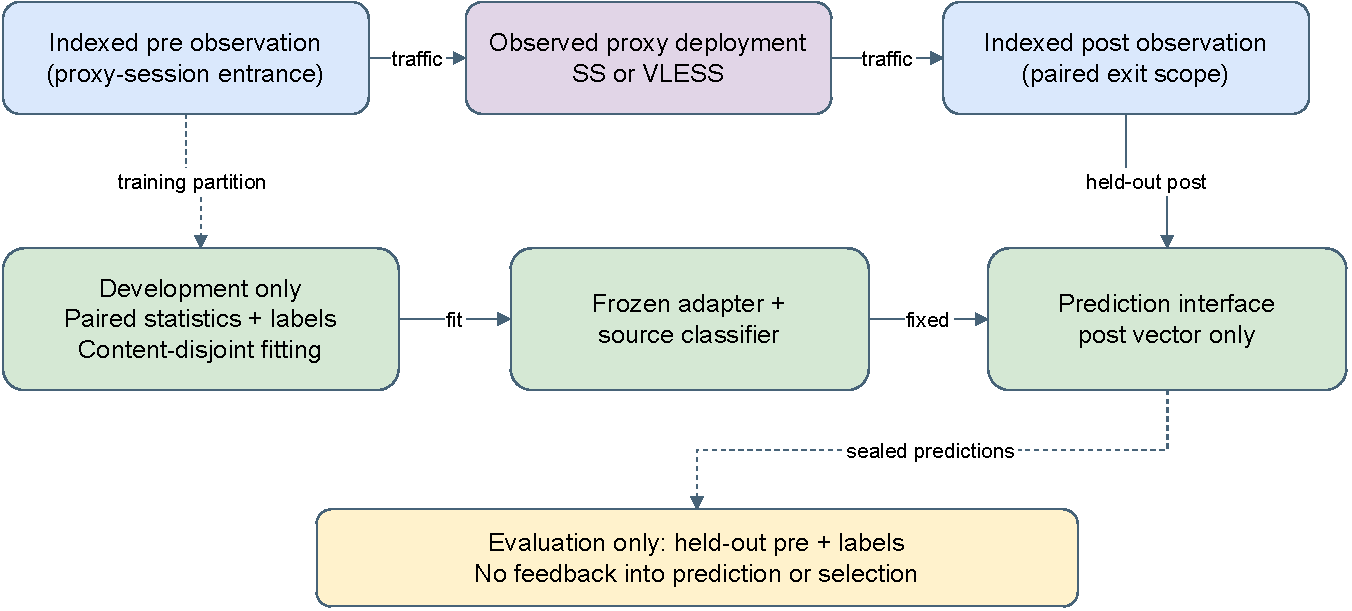
\includegraphics[width=\textwidth]{observation-boundary.pdf}
\caption{Observation and permission boundaries. Indexed paired traffic is available for development. Classification consumes only the selected post vector; labels and test pre remain in an evaluation branch. Offline object selection is retained rather than presented as solved online identification.}
\label{fig:boundary}
\end{figure*}

\subsection{Identity Metadata and Deployment Confounding}
IP addresses, ports, SNI, domain strings, content IDs, and pairing IDs are not predictive input dimensions. Some of these fields are nevertheless necessary to reconstruct entities, assign labels, or audit correspondence. Their absence from model inputs does not imply the absence of deployment cues: packetization, timing, or volume can vary with deployment conditions. SS and VLESS denote the observed deployments, not randomized interventions isolating their protocol specifications. Hy2 measurements in the broader collection use a different carrier scope and are not pooled into the strict TCP classification cohort.

\section{Measurement Design and Motivating Observations}
\subsection{Cohorts and Content-Disjoint Evaluation}
The September 16 collection contains 525 raw visits covering seven candidate business classes. The primary conservative cohort contains 240 visits: 30 contents, two deployments, and four repetitions (collection rounds 1, 2, 4, and 5). A 299-visit sensitivity cohort substantially overlaps this cohort and is not an independent test set. Playback confirmation and eligibility for exclusive TCP correspondence are separate criteria; exclusion from the strict cohort must not be interpreted as proof that playback did not occur.

The September 14 data are retained as historical measurement context. Their strict paired subset contains 140 visits to 14 resources across two deployments and five repetitions. The broader three-deployment collection and this strict subset have different scopes. We do not mix September 14 samples into the primary September 16 training folds or treat their resource-label task as interchangeable with the six-class activity task.

The primary evaluation uses five fixed content-disjoint folds. Each fold has 24 training contents and six held-out contents, producing 192 training and 48 test visits when both deployments are used. All repetitions, both sides, and associated parent visits and connections move with the content. Predictions are pooled across the five held-out folds. The independent content count is 30, not 240. No random packet or connection split is used.

\begin{table}[t]\centering
\caption{Distinct evidence scopes; overlapping cohorts are not independent replications.}\label{tab:cohorts}
\small\begin{tabular}{lrr>{\raggedright\arraybackslash}p{2.7cm}}\toprule
Cohort & Visits & Contents & Role\\\midrule
0914 strict & 140 & 14 & Historical measurement and deployment classification\\
0916 raw & 525 & --- & Collection audit; seven candidate classes\\
0916 primary & 240 & 30 & Six-class model reuse\\
0916 sensitivity & 299 & 30 & Overlapping sensitivity\\\bottomrule
\end{tabular}\end{table}

\subsection{Features and Explicit Packet Semantics}
Packet fields are decoded before custom aggregation; semantic features are not taken from Wireshark's built-in flow statistics. The study distinguishes observed packets from alternative retransmission-filtered interpretations. The measurements here retain observed traffic under the frozen extraction contract. Retransmissions and empty-payload packets can affect some aggregates and are not silently removed.

The classification representation contains 157 dimensions in six groups (Table~\ref{tab:groups}). This is not the complete catalogue of features supported by the extractor. Length distributions use 19 bins, IAT distributions use 23 bins, and the cumulative representation has 101 normalized samples. IATs are computed within original connections; unrelated connections are not joined to create artificial gaps. Distributions and scalar aggregations follow the frozen entity-to-visit contract.

For nonempty packets with direction sequence $(d_1,\ldots,d_N)$, the implemented Flow Reversals run count is
\begin{equation}
 \mathrm{FR}_{\mathrm{runs}}=\begin{cases}0,&N=0,\\1+\sum_{i=2}^{N}\mathbb{1}[d_i\ne d_{i-1}],&N>0.\end{cases}
\end{equation}
The switch count omits the initial one. The classifier's normalized FR coordinate is runs per nonempty packet; the extractor also supports a distinct switches$/ (N-1)$ normalization for $N>1$, which is not substituted for that coordinate. Empty-payload packets are filtered before evaluating FR. In contrast, the observed burst count counts direction runs including empty-payload packets. These are different measurements, even though both describe interaction structure. This operational definition avoids conflating a bidirectional connection with a directional run.

\begin{table}[t]\centering\caption{Frozen classification feature groups.}\label{tab:groups}
\small\begin{tabular}{lp{5.0cm}r}\toprule Group & Scope & Dim.\\\midrule
G1 & Transport/IP and directional byte volume & 4\\
G2 & Upstream byte share, direction entropy & 2\\
G3 & FR and directional transitions & 4\\
G4 & Packetization, bursts, length distribution & 22\\
G5 & Median IAT and IAT distribution & 24\\
G6 & Normalized cumulative traffic shape & 101\\\bottomrule\end{tabular}
\end{table}

\subsection{Repeatable Changes Without Universal Invariance}
For positive scalar measurements, define $\Delta_{u,r,c}=\ln(x^+_{u,r,c}/x^-_{u,r,c})$, where $u,r,c$ index content, repetition, and deployment. We first summarize repetitions within a content and then summarize contents with equal weight. A typical ratio is the exponential of the median of content-wise median log ratios. It is neither the ratio of total bytes nor a pooled connection median. Within-content MAD is unscaled; IQR uses linear quantiles. These are descriptive repeatability statistics, not ICC estimates.

Figure~\ref{fig:transform} contrasts typical changes with repetition dispersion. In SS, packet count and observed bursts have typical ratios 1.6746 and 1.7509, while transport-payload bytes have ratio 1.0196. All 30 content medians exceed 1.1 for packet and burst counts. VLESS exhibits a smaller packet ratio of 1.2453 but a larger FR ratio of 1.2303 than SS (1.0561). VLESS bursts are heterogeneous: 13 content medians exceed 1.1, 13 lie in $[0.9,1.1]$, and four are below 0.9. The reference band is descriptive, not an equivalence test.

\begin{figure*}[t]\centering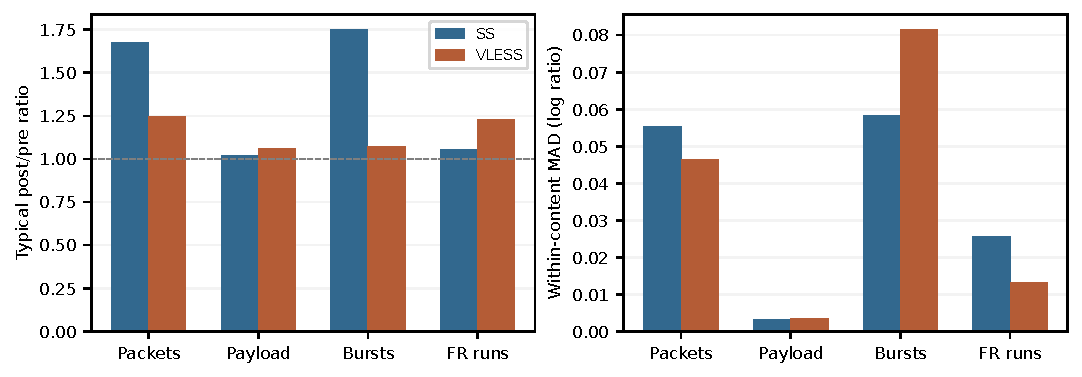
\includegraphics[width=\textwidth]{transformations.pdf}
\caption{Primary-cohort transformations. Left: typical post/pre ratios computed by nested content/repetition medians. Right: median within-content MAD of natural-log ratios. The right panel describes repeat dispersion, not uncertainty intervals for the left panel.}\label{fig:transform}\end{figure*}

Length and IAT changes are summarized by Jensen--Shannon divergence in bits, not its square-root distance. SS typical divergences are 0.3509 and 0.1973, compared with 0.0627 and 0.0783 for VLESS. Positive divergence does not specify a direction of change. In the 299-visit sensitivity cohort the major descriptive directions persist. Five resources overlap the two strict collection batches, but matching a resource does not match network conditions, action duration, or returned content. Historical agreement supplies contextual replication, not an external blinded validation.

\subsection{Recoverability and Task Utility Do Not Rank Together}
We compare a fixed one-dimensional Ridge recovery baseline for each feature with fixed post-side logistic classifiers trained on each group alone and on all groups except that group. These are separate fitted learners under the same content partition, not zeroing dimensions of a fitted model. Recovery skill is $1-\mathrm{MSE}_{\mathrm{model}}/\mathrm{MSE}_{\mathrm{train\ mean}}$ under the frozen content-weighted evaluation. Negative values are retained.

Figure~\ref{fig:groups} reveals a mismatch. G1 has recovery skill 0.9933 but only-group macro-F1 0.5711; G4 has skill 0.3036 but only-group macro-F1 0.8150. Removing G4 reduces full-feature F1 by 0.0662, with a descriptive interval $[0.0336,0.0995]$. G6 is highly recoverable (0.9879), yet its deletion increment is not clearly positive. These comparisons do not estimate mutual information or model-independent unique contributions. They motivate testing the recovery objective directly while keeping the source classifier and mapping capacity fixed.

\begin{figure*}[t]\centering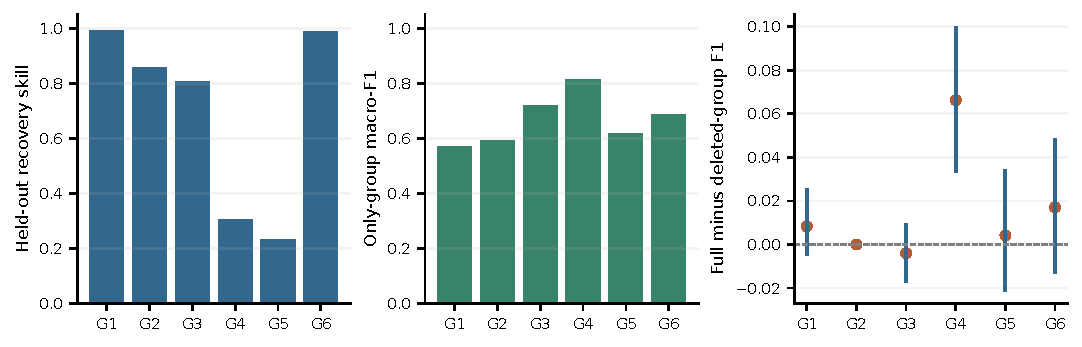
\includegraphics[width=\textwidth]{group-utility.pdf}
\caption{Distinct group diagnostics: held-out univariate recovery skill, single-group post classification, and full-minus-deleted-group F1. Only the last panel includes 95\% paired content-bootstrap intervals. Shared group names do not make the vertical quantities interchangeable.}\label{fig:groups}\end{figure*}

\section{Controlled Model-Reuse Framework}
\subsection{Fixed Source Classifier and Coordinates}
Let $x^-$ and $x^+$ denote the pre and post visit vectors. Training-only median imputation and standardization define $z^-=T^-(x^-)$ and $v=T^+(x^+)$. The source classifier is
\begin{equation}
 h^-(z)=\operatorname{softmax}(Wz+\beta),\quad K=6.
\end{equation}
It is a multinomial logistic regression with fixed L2 regularization, $C=1$, LBFGS, tolerance $10^{-8}$, and at most 10,000 iterations. There is no class weighting or hyperparameter search. The classifier remains fixed across A--D and F--H within a fold. Method E independently fits the same classifier family on post training data.

The original statistical target uses a separately recorded training normalization $t^-=U^-(x^-)$. To reproduce that objective exactly, the adapter first outputs $q=a\odot v+b$ in the $U^-$ coordinates and then converts it to source coordinates,
\begin{equation}\widehat z^-=c\odot q+d_0.\label{eq:coordinate}\end{equation}
The conversion coefficients are determined from training preprocessing, not fitted on held-out samples. Constant or unusable pre target dimensions are excluded from recovery fitting, and their source-coordinate values follow the stored constant-dimension rule. The observed Full representation has 149 effective recovery dimensions and 298 affine parameters. E retains its own post information; it is not artificially restricted by the pre recovery mask.

Direct transfer B applies the source preprocessing $T^-$ to raw post features. It does not replace the source scaler with a test-post scaler. Calibrated methods use training-fitted $T^+$ followed by Eq.~\eqref{eq:coordinate}. This distinction prevents the apparent success of a method from being caused by mixing standardized coordinate systems.

\subsection{Statistical and Decision-Aware Calibration}
For training target $t_i$ and $d=149$, the statistical objective is
\begin{equation}
 L_{\mathrm{rec}}=\frac{1}{nd}\left[\sum_{i=1}^{n}\|a\odot v_i+b-t_i\|_2^2+\alpha\|a\|_2^2\right],\label{eq:rec}
\end{equation}
with $\alpha=1$. The intercept is unpenalized. Missingness and effective-dimension handling reproduce the stored recovery contract; the main cohort supplies complete evaluated targets. The $n$ and $d$ factors are retained rather than silently changing the regularization scale.

Let $P_K=I_K-\boldsymbol{1}\boldsymbol{1}^{\mathsf T}/K$. For a target source vector $z_i^\star$, define
\begin{equation}
 L_{\mathrm{dec}}=\frac{1}{n(K-1)}\sum_i\|P_KW(\widehat z_i^--z_i^\star)\|_2^2.
\end{equation}
Decision-aware calibration minimizes $L_{\mathrm{rec}}+\lambda L_{\mathrm{dec}}$ with the same diagonal affine mapping. The primary setting is $\lambda=1$; previously specified values 0.1 and 10 are sensitivity analyses, not opportunities to select a target-domain winner. The $\lambda=0$ implementation reproduces C/D numerically. The objective is quadratic in $(a,b)$ because $W$ is frozen, although the decision term couples coordinates in the optimization. Coupled optimization does not add cross-coordinate terms to the inference mapping.

The source classifier was trained with activity labels. Consequently, this is \emph{task-aware} calibration even though the added term reads source scores rather than explicit labels. ``Unsupervised'' would conceal an important source of supervision. Figure~\ref{fig:framework} separates fitting from inference.

\begin{figure*}[t]\centering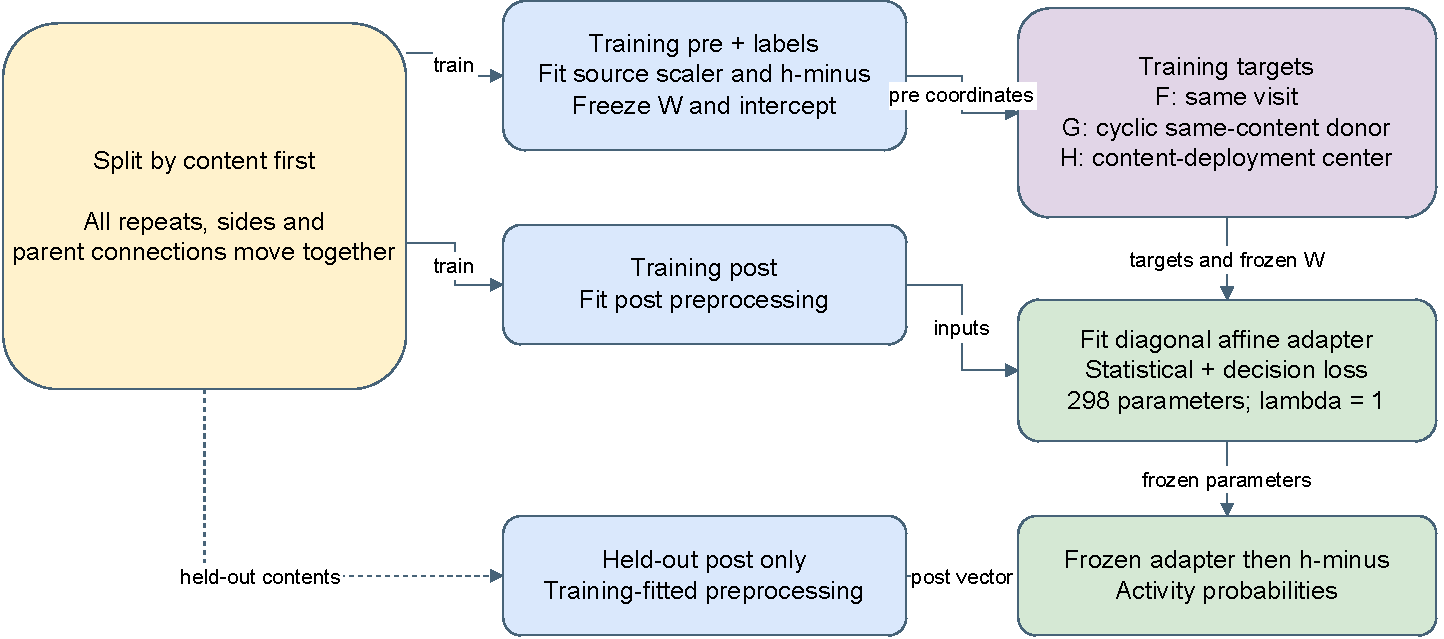
\includegraphics[width=\textwidth]{calibration-framework.pdf}
\caption{Controlled calibration workflow. Target construction occurs only within outer training contents. F/G/H retain the same affine capacity and frozen source classifier. H does not look up a content center at inference.}\label{fig:framework}\end{figure*}

\subsection{Correspondence Controls}
Table~\ref{tab:arms} defines the eight arms. C/F use same-visit targets. D/G assign each input a frozen non-self cyclic donor within the same content and deployment, retaining four inputs and four targets. This donor is not an independent draw from a conditional distribution. H assigns all training inputs within a content--deployment group its mean pre target. Both recovery and decision targets change together. Post inputs are not averaged; H learns one global map and receives neither content identity nor centers at inference.

\begin{table*}[t]\centering\caption{Controlled arms and resource requirements. All classifiers use activity supervision; F/G/H additionally use the resulting source weights in the calibration loss.}\label{tab:arms}
\small\setlength{\tabcolsep}{5pt}\begin{tabular}{llll}\toprule
Arm & Classifier & Calibration resource/objective & Actual test input\\\midrule
A & Fixed pre classifier & None; diagnostic reference & Held-out pre\\
B & Same pre classifier & None & Raw post through source preprocessing\\
C & Same pre classifier & Same-visit pairs; statistical recovery & Mapped post\\
D & Same pre classifier & Cyclic same-content donor; statistical recovery & Mapped post\\
E & Independently fitted post classifier & Post training labels & Post\\
F & Same pre classifier & Same-visit pairs; recovery + decision & Mapped post\\
G & Same pre classifier & Cyclic donor; recovery + decision & Mapped post\\
H & Same pre classifier & Content--deployment centers; recovery + decision & Mapped post\\\bottomrule
\end{tabular}\end{table*}

Exact pairs can themselves be coarsened into H targets. Therefore, a benefit of H would concern how correspondence is used, not a theorem that less available information is better. Furthermore, exact pairs allow pre labels to be transferred to post for E. We have not established a reduction in annotation cost. The controlled question is preservation of an existing source decision rule under a restricted adapter, not whether calibration dominates retraining with the same label resources.

\subsection{Source-Only Cross-Deployment Fitting}
For each direction and outer fold, only the source deployment's 96 training visits from 24 contents fit preprocessing, classifiers, and F/H. The same six held-out contents yield 24 source and 24 target visits. The target deployment's remaining 96 visits are registered as forbidden fitting members, not used for adaptation. Each direction has its own models and scalers. E becomes $E_s$, a post classifier trained only in the source deployment, not the jointly trained E or a target-supervised oracle.

All ten contexts retain 149 recovery dimensions and 298 parameters. The experiment adds 20 logistic classifiers and 20 adapters, with no neural training. Alpha and C remain fixed when training size decreases from 192 to 96. For this reason, changes from old jointly trained models cannot be attributed solely to deployment shift. The principal shift comparison uses the \emph{same newly fitted model} on source and target held-out contents.

\section{Analytical Interpretation}
This section gives standard identities and elementary consequences that organize the experiments. They are not claims of a new information-theoretic bound or empirical estimates of mutual information.

\subsection{Accessible Prediction Is Not Additional Shannon Information}
Let $(A,B,Y,U)\sim\mathcal P_c$ denote pre features, post features, label, and content in deployment $c$. We do not assume $A\perp c$ or a Markov chain $Y\to A\to B$. Under a fixed trained mapping $Z=r_\theta(B)$ and independently evaluated data, the data-processing inequality gives
\begin{equation}I(Y;Z\mid\theta)\le I(Y;B\mid\theta).
\end{equation}
A classifier can nevertheless perform better on $Z$ because the representation is more compatible with its restricted decision rule. This motivates a finite-learner interpretation, consistent with computationally constrained information frameworks~\cite{vinfo}, rather than claiming that calibration creates Shannon information.

For a normalized predictor $q$ and logarithms of base two,
\begin{align}
 \E[-\log_2 q(Y\mid B)]&=H(Y\mid B)\nonumber\\
 &\quad+\E_B D_{\mathrm{KL},2}(P(Y\mid B)\|q(Y\mid B)).
\end{align}
The equality concerns population, uncapped cross-entropy. Empirical CE, finite fitting error, and probability-floor clipping are separate issues. Neither CE differences nor recovery skill are reported as mutual information or predictive $\mathcal V$-information. Conditional information such as $I(Y;A\mid B)$ remains a conceptual question, not an estimated result.

\subsection{Recovery and Decision Geometry}
The source posterior depends on relative logits. If $P_KW(\widehat z-z)=0$, the two logit vectors differ by a common scalar and their softmax probabilities agree. This does not require $\widehat z=z$. The centered projection has rank at most $K-1$, but this algebraic fact does not imply that all business information has five intrinsic dimensions.

In common source coordinates, write recovery distortion as $e^{\mathsf T}Q_{\mathrm{rec}}e$ and decision distortion as $\|P_KWe\|^2/(K-1)$. Then the combined quadratic metric is
\begin{equation}
 M=Q_{\mathrm{rec}}+\frac{\lambda}{K-1}W^{\mathsf T}P_KW.
\end{equation}
If $z=Ct+d_0$, then $Q_{\mathrm{rec}}=C^{-\mathsf T}C^{-1}/d$ on effective coordinates. It reduces to $I/d$ only when the relevant scales agree. Keeping this metric and the transformed slope regularizer explicit is necessary to preserve Eq.~\eqref{eq:rec}.

\subsection{What a Center Target Removes}
For equal-weight, complete targets within group $g$, let $a_i=\mu_g+\epsilon_i$, $\sum_{i\in g}\epsilon_i=0$, and let $q_i$ be the prediction in the same coordinates. With fixed $M$, the instance-minus-center data-loss difference is
\begin{align}
 L_{\rm inst}-L_{\rm center}
 &=\frac1n\sum_i\epsilon_i^{\mathsf T}M\epsilon_i\nonumber\\
 &\quad-\frac2n\sum_g\sum_{i\in g}(q_i-\overline q_g)^{\mathsf T}M\epsilon_i.\label{eq:center}
\end{align}
The common regularizer cancels. Thus instance targets additionally reward alignment with group-centered target residuals. This is not a decomposition into causal signal and noise. Averaging squared error over \emph{all} possible within-group targets is equivalent, up to a prediction-independent constant, to using the center. A single cyclic donor does not perform that averaging and is not identical to H.

\subsection{Separating Deployment and Calibration Risks}
Let $R_s^-$ be source-entrance 0--1 risk, $R_t^-$ the same classifier's target-entrance risk, and $R_t^+$ its risk on mapped target post. The accounting identity
\begin{equation}
 R_t^+=R_s^-+(R_t^--R_s^-)+(R_t^+-R_t^-)
\end{equation}
separates two comparisons without claiming causal attribution; either difference may be negative. It is not an identity for macro-F1.

For completeness, let $m(A_t)$ be the top-two margin of $WA_t+\beta$, $e=r(B_t)-A_t$, and $D=\E\|P_KWe\|_2^2<\infty$. For any $\tau>0$, deterministic tie-breaking and the pairwise score perturbation bound give
\begin{equation}
 R_t^+\le R_t^-+P(m(A_t)\le\tau)+\frac{2D}{\tau^2}.\label{eq:margin}
\end{equation}
Indeed, outside the small-margin event a changed winner requires $\|P_KWe\|_2\ge\tau/\sqrt2$; Markov's inequality bounds that event. The bound can be loose and requires offline target-pre information. It is explanatory, not a deployment-time certificate. Here $D$ is unnormalized; it is five times the reported six-class centered-logit MSE under matching averaging. Target-pre accuracy is also not an upper bound: a map may change an incorrect source decision into a correct one.

\section{Evaluation}
\subsection{Protocol, Metrics, and Uncertainty}
All main comparisons use the frozen five-fold content partition and Full157 features. Fits use CPU float64 with one numerical thread in the Pytorch312 environment. The final calibration experiments do not require CUDA or neural optimization. F1 is macro-averaged across the six classes; CE uses base-two logarithms and the inherited probability floor of $10^{-15}$; Brier is the sum of squared class-probability errors; balanced accuracy averages class recall. Pooled F1 is computed from pooled out-of-fold predictions, not by averaging deployment F1 values.

Paired comparisons use 2,000 bootstrap resamples of contents, stratified by business class, with seed 20260919. All visits belonging to a sampled content move together. Reported 95\% intervals are unadjusted and conditional on the fitted models: the bootstrap does not retrain models or account for historical method selection. The five training folds overlap and are not five independent experimental repetitions. Unless otherwise specified, positive CE gain means baseline loss minus candidate loss, whereas positive F1 gain means candidate F1 minus baseline F1.

The pipeline retains member and provenance checks, separated prediction/evaluation inputs, and numerical replay. In the cross-deployment stage, 20 independent augmented-QR checks agree with fitted adapters to a maximum parameter difference of $3.26\times10^{-14}$; replay of 2,400 predictions has maximum numerical difference $3.27\times10^{-13}$ and identical classes. These are implementation checks, not evidence of population generalization. Existing connection-identity audits are reused; this paper build does not perform another full raw-packet scan.

\subsection{Direct Transfer and Statistical Calibration}
Table~\ref{tab:ah} and Fig.~\ref{fig:ah} report A--H. The source classifier performs well on held-out pre (A: \FOneA{}) but poorly on post passed through the same source preprocessing (B: \FOneB{}). Switching A to B turns 117 of 240 previously correct predictions into errors and corrects only one previously incorrect prediction. This is a decision-level failure, not merely a change in average feature magnitude.

\begin{table}[t]\centering\caption{Joint-deployment, content-held-out results. F1 is macro-F1; BA is balanced accuracy.}\label{tab:ah}
\small\begin{tabular}{lrrrr}
\toprule
Arm & F1 & CE (bits) & Brier & BA \\
\midrule
A & 0.9547 & 0.2440 & 0.0785 & 0.9542 \\
B & 0.4555 & 4.8548 & 0.8996 & 0.4708 \\
C & 0.7687 & 0.9264 & 0.3231 & 0.7708 \\
D & 0.6458 & 1.1962 & 0.4312 & 0.6500 \\
E & 0.9082 & 0.5234 & 0.1611 & 0.9083 \\
F & 0.8535 & 0.6549 & 0.2192 & 0.8542 \\
G & 0.8656 & 0.6550 & 0.2217 & 0.8667 \\
H & 0.8646 & 0.6231 & 0.2073 & 0.8667 \\
\bottomrule
\end{tabular}
\end{table}
\begin{figure*}[t]\centering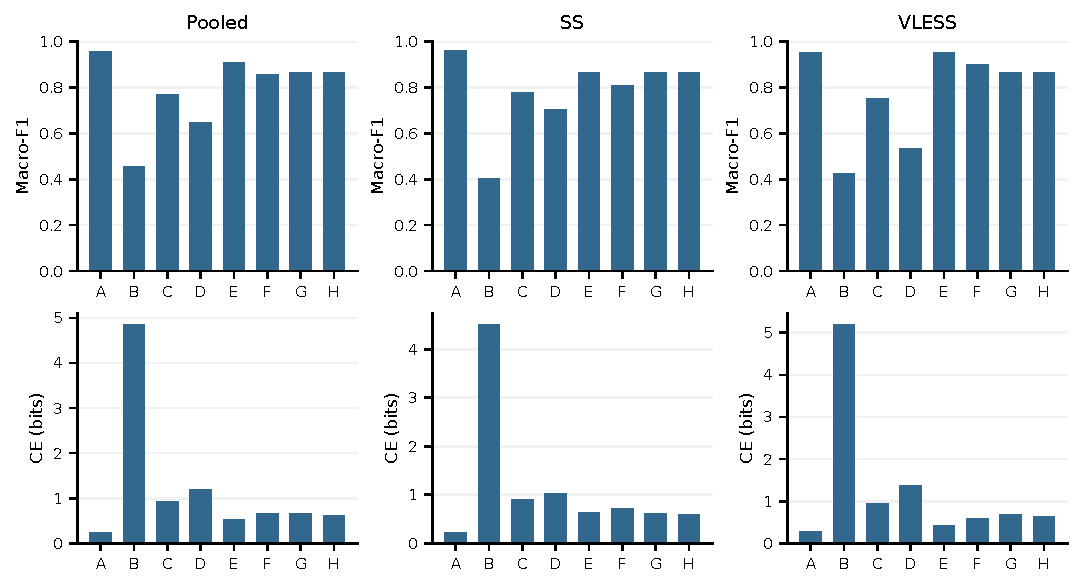
\includegraphics[width=\textwidth]{ah-performance.pdf}
\caption{A--H under pooled and deployment-specific evaluation. Each panel uses the same held-out visits within its scope. The high direct-transfer loss is retained; probability and classification metrics are not conflated.}\label{fig:ah}\end{figure*}

Statistical calibration C restores F1 to \FOneC{}. Its gain over B is 0.3132, with interval $[0.2469,0.3813]$. C also exceeds cyclic-mismatch D by 0.1229, interval $[0.0777,0.1719]$. Therefore precise correspondence has observable value for this recovery objective. However, C remains below pre-reference A and post-supervised E (\FOneE{}). From B to C, 96 errors are corrected and 24 correct predictions are lost. A low-dimensional mapping thus offers partial reuse, not complete recovery of source decisions.

\subsection{Changing the Objective Without Increasing Capacity}
Adding the centered-logit term gives F1 \FOneF{} for F, a gain of 0.0848 over C with interval $[0.0552,0.1195]$. CE decreases from 0.9264 to 0.6549 bits, and its improvement interval is also positive. This comparison fixes the source classifier, affine capacity, training visits, and principal coordinates; the intervention is the calibration objective.

Crucially, F's statistical MSE increases from 0.2200 to 0.3737, while centered-logit MSE decreases from 3.7327 to 2.4400. Figure~\ref{fig:tradeoff} and Table~\ref{tab:fidelity} show that prioritizing decision-related directions can improve business prediction while sacrificing average statistical fidelity. This is a controlled method comparison, not a causal regression of F1 against MSE.

\begin{figure*}[t]\centering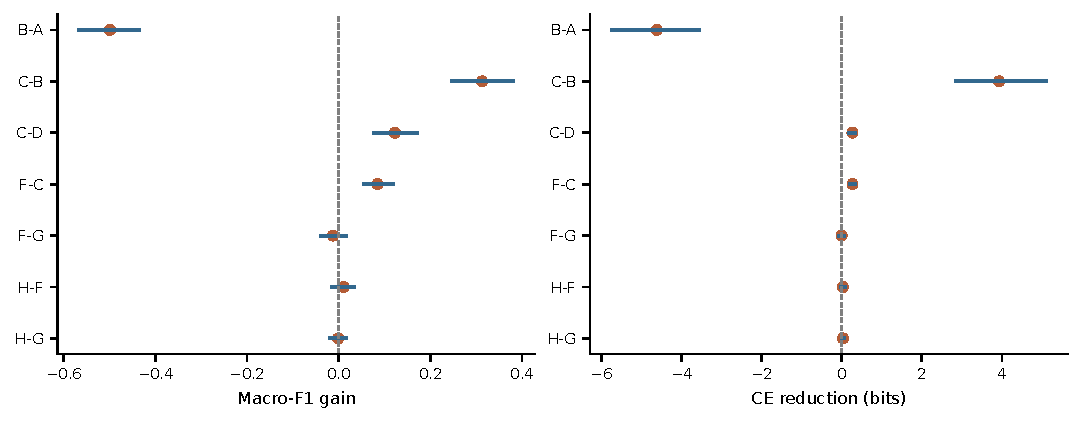
\includegraphics[width=\textwidth]{paired-contrasts.pdf}
\caption{Selected frozen comparisons: point estimates and paired content-bootstrap intervals. F1 gains and CE reductions have different units. Intervals are descriptive, unadjusted, and conditional on fitted models; crossing zero does not establish equivalence.}\label{fig:contrasts}\end{figure*}
\begin{figure*}[t]\centering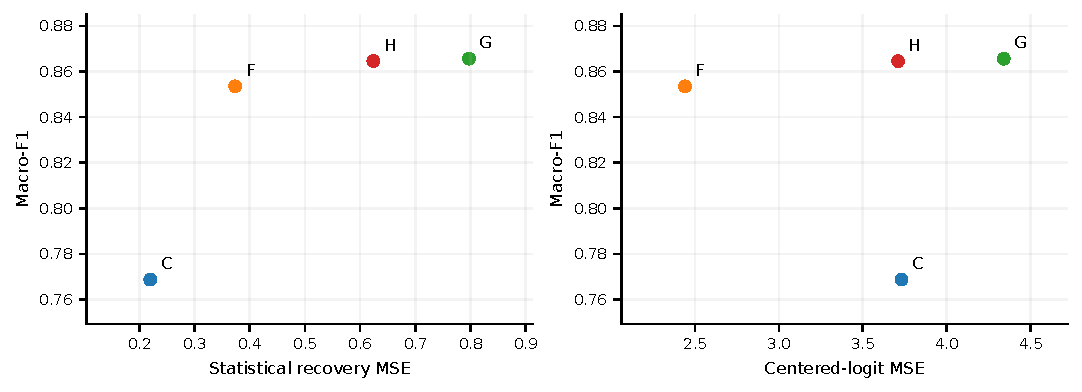
\includegraphics[width=\textwidth]{recovery-task.pdf}
\caption{Statistical and source-score recovery versus task performance for C/F/G/H. Each point is a complete method, not an independent sample from a fitted trend. Lower reconstruction error does not induce a universal ranking of macro-F1.}\label{fig:tradeoff}\end{figure*}
\begin{table}[t]\centering\caption{Held-out recovery against true same-visit pre; agreement is with A's predicted class, not the true label.}\label{tab:fidelity}
\small\begin{tabular}{lrrr}
\toprule
Arm & Stat. MSE & Logit MSE & Agreement \\
\midrule
C & 0.2200 & 3.7327 & 0.7875 \\
F & 0.3737 & 2.4400 & 0.8583 \\
G & 0.7974 & 4.3419 & 0.8542 \\
H & 0.6240 & 3.7111 & 0.8542 \\
\bottomrule
\end{tabular}
\end{table}

Yet F does not clearly exceed G, which has F1 \FOneG{} and CE 0.6550. The pooled F--G intervals cross zero for both metrics. This does not invalidate C's advantage over D: instead, the use of precise pairing changes with the objective. The observed improvement cannot be attributed entirely to exact visit correspondence. Results at $\lambda=0.1$ and 10 are retained in the supplement without selecting a new primary setting after seeing outcomes.

\subsection{Changing Correspondence Granularity}
H predicts content--deployment centers during fitting and obtains F1 \FOneH{} and CE 0.6231. H--F has F1 difference 0.0111 with interval $[-0.0135,0.0336]$; H--G is $-0.0010$ with interval $[-0.0185,0.0170]$. No equivalence margin was specified, so these are inconclusive superiority comparisons, not equivalence results. H's lower CE than G has interval $[0.0079,0.0611]$, but this probability-loss result does not establish classification superiority.

H has statistical MSE 0.6240 and logit MSE 3.7111, both worse than F. Coarser targets therefore sacrifice visit-level recovery without a commensurate pooled classification decline in this task. Within the outer training groups, all four repetitions have identical source-predicted classes, although their source scores differ. That observation is training-only: the source classifier is also 100\% correct there, and the result must not be generalized to held-out repetition agreement.

Deployment-specific results prevent a stronger conclusion. In SS, H's F1 is 0.8636 versus F's 0.8075; in VLESS, H is 0.8640 versus F's 0.8994, and F has better probability metrics. Averaging these patterns would conceal an important exception. Moreover, center targets change target dispersion as well as matching granularity. The experiment does not isolate a pure information quantity attached to instance identity.

\subsection{Cross-Deployment Reuse}
Figure~\ref{fig:cross} contrasts source and target holdouts for the same source-only models; complete values are in the supplement. In SS-to-VLESS, A/B/F/H/$E_s$ have target F1 0.3032/0.3503/0.3356/0.3685/0.4476. Neither F nor H shows a positive F1 interval relative to B, although both reduce CE substantially. In VLESS-to-SS, corresponding F1 values are 0.4299/0.3653/0.5538/0.6059/0.3740. F--B gains 0.1885 with interval $[0.0803,0.3131]$; H--B gains 0.2406 with interval $[0.1142,0.3673]$. Both also improve over $E_s$ in that direction.

\begin{figure*}[t]\centering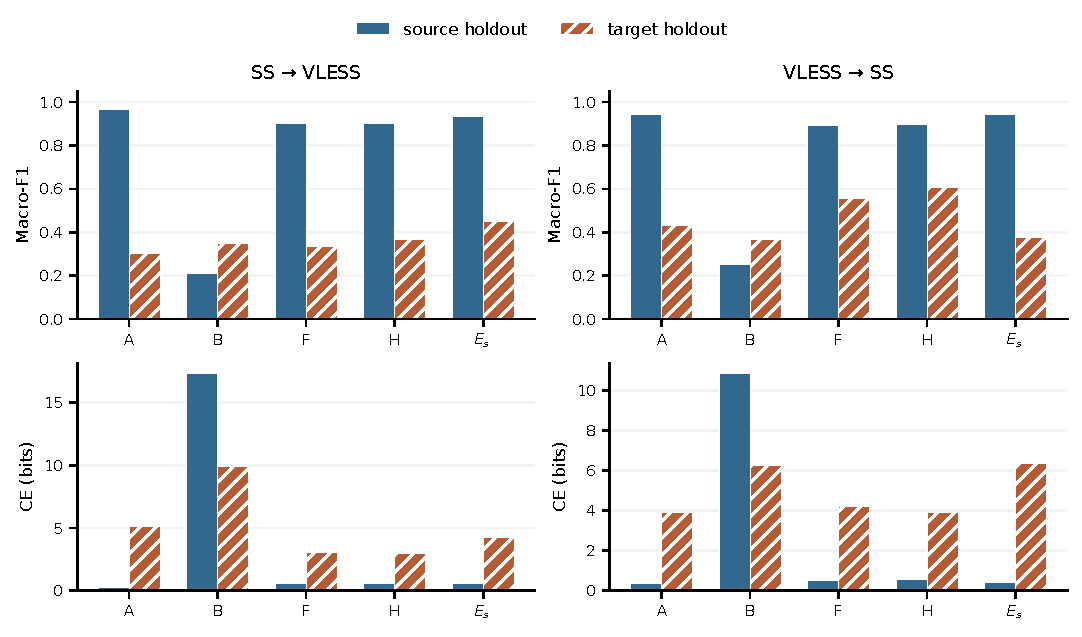
\includegraphics[width=\textwidth]{cross-deployment.pdf}
\caption{Source-only fitting followed by source and target content-held-out evaluation. Models and preprocessing are identical across the two bars for each arm. $E_s$ is trained on source post labels only. CE uses the frozen probability-floor convention.}\label{fig:cross}\end{figure*}

The source-side limitation is pronounced. An SS-trained pre classifier has F1 0.9666 on held-out SS pre and 0.3032 on target VLESS pre. The reverse direction drops from 0.9416 to 0.4299. The bootstrap intervals for both differences are negative. Thus the adapter is not the only transfer bottleneck: the fixed source decision rule is itself deployment-dependent. This evidence supports an additional constraint on fidelity-based reuse, not a proof that all useful adaptation must reproduce target pre exactly.

Figure~\ref{fig:changes} illustrates decision-level effects. In SS-to-VLESS, B-to-F fixes 26 errors but introduces 28; B-to-H fixes 27 and introduces 22. In VLESS-to-SS, B-to-H fixes 36 and introduces 13. The latter benefit is not universal across classes: Bing does not share the aggregate improvement. Likewise, the SS-to-VLESS YouTube classes remain difficult. The supplement reports per-class results rather than letting a favorable class conceal failure elsewhere.

\begin{figure*}[t]\centering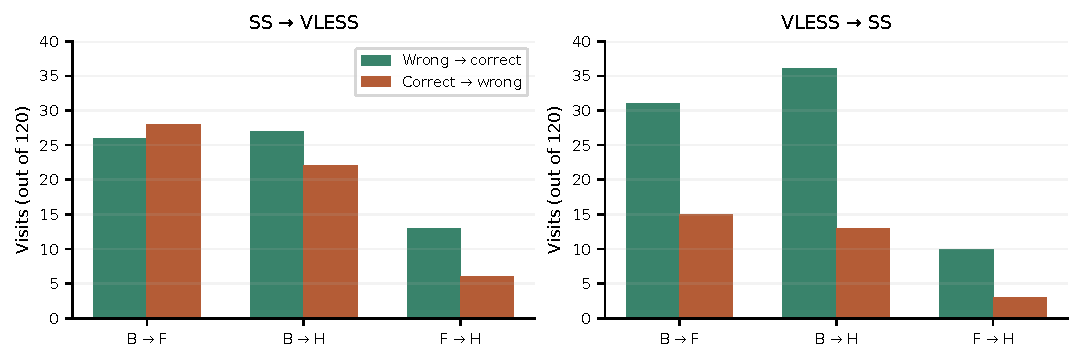
\includegraphics[width=\textwidth]{decision-changes.pdf}
\caption{Repairs and newly introduced errors on the same target visits. Different deployments are never paired as if they were the same capture. Wrong-to-wrong class changes are excluded from both categories.}\label{fig:changes}\end{figure*}

F/H target CE remains above the uniform six-class value $\log_2 6\approx2.585$ in both directions. Thus F1 gains do not imply well-calibrated probabilities. Uncapped logit CE is retained separately: VLESS-to-SS F/H each has one probability-floor event, yielding uncapped CE 4.2632/3.9726 rather than reported 4.2131/3.9222. This matters for interpreting highly confident mistakes.

\subsection{Relationship to Earlier Learning Experiments}
Earlier work in this project examined distillation, natural-pair SSL, and group-recovery objectives. They are not a chronological sequence culminating in a universally stronger H. Six-class natural-pair fine-tuning achieved F1 0.9018 versus supervised 0.9017 without a clear joint F1/CE gain. Conversely, a local two-class YouTube MLP experiment with the 157-dimensional representation improved SS-to-VLESS F1 from 0.3440 to 0.5811 with a pre teacher and exceeded ordinary post and mismatched controls. These distinct setups demonstrate both a local positive result and limits to generality. They cannot be pooled with A--H as a common leaderboard or used to dismiss paired learning as a whole.

\section{Related Work}
\subsection{Encrypted Traffic Inference and Correlation}
Website-fingerprinting studies such as Deep Fingerprinting~\cite{df} and automated feature learning~\cite{automated} establish that encrypted traffic can support website inference with learned representations. Their attack tasks and observation regimes differ from reuse of a fixed entrance-side classifier on paired exit-side aggregates. We do not compare their published accuracy with our six-class activity F1: the class spaces, data volumes, defenses, and evaluation settings are not matched.

DeepCorr~\cite{deepcorr} learns to associate network flows across Tor. It is relevant because it treats correspondence as learnable structure rather than relying solely on generic correlation statistics. Our target is different: correspondence is supplied by the collection process during training, and the inference output is an activity class rather than a match between two observed flows. We therefore study the usefulness of known relationships under a one-sided classifier interface, not a replacement for flow correlation.

\subsection{Paired Learning and Task-Aware Adaptation}
Knowledge distillation~\cite{distill} transfers predictive behavior through teacher outputs, whereas contrastive learning~\cite{simclr} learns representations through view relationships. Work on view selection emphasizes retaining task-relevant information rather than treating shared information as sufficient~\cite{views}. These ideas motivate our controls, but the final experiment uses neither a new neural student nor a larger representation network. Its calibrated vector is optimized against a frozen source decision rule with a quadratic objective.

Studies of invariant representations in domain adaptation show that feature alignment and source-domain success alone do not guarantee target success~\cite{zhao}. Our directional evaluation is compatible with that warning, but does not empirically identify every assumption of those theoretical results. In particular, our balanced cohort is not evidence of marginal label shift. We distinguish an observed source-entrance failure from a claim about the unique cause of domain shift.

\subsection{Information and Finite-Learner Utility}
Predictive $\mathcal V$-information formalizes informativeness relative to computational constraints~\cite{vinfo}. We use the distinction between information availability and accessibility to organize the experiments. We do not implement its estimator or claim that a difference between two empirical losses equals a general information quantity. Our contribution is a controlled traffic study showing that reconstruction, decision preservation, and cross-deployment classification need not have the same ordering.

\section{Discussion and Limitations}
\subsection{What the Evidence Supports}
The observed traffic has structured correspondence, and a fixed classifier can benefit from an appropriately chosen calibration objective. However, the benefit is conditional on label, representation, deployment, and available correspondence. The fact that F does not exceed G/H in the pooled setting is not a reason to erase C's advantage over D; nor does the latter establish a universal requirement for exact instance targets. These results address different objectives under a deliberately restricted mapping family.

The apparent simplicity of logistic regression is useful for this question: frozen logits make the added objective explicit, and affine mappings make numerical replication straightforward. It is also a limitation. Results for fixed statistics and a restricted adapter do not establish the best attainable performance of sequence models, nonlinear maps, or arbitrary post-only learners. Earlier MLP evidence is retained precisely to avoid equating a limited model-family result with an impossibility statement.

\subsection{Physical Validity and Supervision Cost}
Adapter outputs can violate nonnegativity, histogram bounds, or cumulative-curve monotonicity. No clipping or projection was added after observing results. These vectors are task-adapted coordinates, not physically valid reconstructed traffic, and the results do not establish reversible proxy transformations. Task benefit and physical plausibility are different requirements.

F/G/H inherit label information through $W$. H also requires knowing which training observations share content and deployment, even without visit-level pairing. Moreover, exact correspondence permits transferring pre labels to post and fitting E. Consequently, the experiments demonstrate reuse under a fixed source model, not a proven annotation saving over all alternatives. Deployment-ready savings in labeling, computation, or collection effort require a separately specified cost model.

\subsection{Validity and Generalization}
Only two existing strict TCP deployments enter the main task. Protocol, server, implementation, path, and collection conditions are not independently randomized. Historical measurements across September 14 and 16 do not remove those confounders. The source-only experiment excludes target numerical data from fitting, but both deployments have already been used to develop the research direction. This is not a fresh external blind test.

The cohort contains only five contents per class, and most labels distinguish domains as well as activity. It is a closed-set visit-level study. The intervals condition on saved models and are not adjusted for the many historical analyses. They do not capture model-selection uncertainty or future environment shifts. No prespecified equivalence margin supports calling F/G/H equivalent. Repeated visits and overlapping sensitivity cohorts do not increase the number of independent contents.

Engineering audits reduce specific leakage risks, including splitting a content's paired observations across fitting and testing. They do not prove that every possible environmental shortcut has been eliminated. Excluding identity fields prevents one direct shortcut but cannot remove deployment-related structure already encoded in traffic statistics. Likewise, a prediction interface that rejects test pre does not make the offline object-selection step an operational attack.

\subsection{Ethics, Reproducibility, and Scope}
This reference draft reports existing research captures and introduces no additional interception or deployment. Packet captures and identity metadata are not embedded in the manuscript artifact; figures are regenerated from aggregate saved results. A public release should review payload and endpoint sensitivity, collection authorization, and any applicable institutional requirements. Formal ethics approval, participant consent, or unrestricted data-release rights are not asserted without author confirmation.

The accompanying artifact records source hashes and generates empirical plots and tables without fitting models. The remaining unvalidated settings include true direct-to-proxy transfer, single-flow classification, index-free online segmentation, and new VPS, network, date, or client environments. These are boundaries of the present evidence rather than capabilities implied by a high closed-set score.

\section{Conclusion}
Traffic correspondence across a proxy boundary is a useful measurement and learning resource, but its utility depends on the downstream decision and deployment. In the observed cohort, statistical calibration partly restores a fixed source classifier, and decision-aware calibration improves classification without improving full statistical recovery. Coarsening training targets changes reconstruction fidelity and deployment-specific outcomes without a corresponding pooled classification collapse. Source-only cross-deployment evaluation exposes an additional limitation: the entrance classifier itself does not remain reliable across deployments. The evidence supports a task-dependent account of cross-side model reuse, not universal benefits of exact pairing or a deployment-independent attack. Future validation requires genuinely external environments and observation models that do not rely on offline object selection.
\bibliographystyle{IEEEtran}
\bibliography{references}
\end{document}
